\chapter{Polynomial Commitment Schemes}
En la sección \ref{sec:oraculos} definimos a los oráculos como un objeto matemático casi mágico. En la práctica, por supuesto, esto no es así, sino que son implementados a través de un protocolo interactivo entre el prover y el verifier. Muchas de las propiedades de los SNARKs se derivan directamente de las propiedades que proveen estos protocolos, como los tamaños de las pruebas. La familia de protocolos para resolver el problema de los oráculos se conoce como \textbf{\textit{Polynomial Commitment Scheme}}. La idea general es la descrita anteriormente, pero ahora vamos a dar una idea un poco más bajo nivel.

Un prover posee un polinomio privado y un verifier quiere conocer la evaluación de este polinomio en un punto. Los Polynomial Commitment Schemes son una herramienta que permite a un prover \textbf{comprometerse} a un polinomio, de manera tal que el verifier pueda hacer consultas sucesivas sobre sus valores en cualquier punto $z$ del dominio de la función asociada y obtener un resultado que puede estar convencido de que se corresponde con la evaluación de la función asociada a ese polinomio en $z$.

La interfaz de estos protocolos está compuesta por 3 funciones:
\begin{enumerate}
    \item $Commit(p) \rightarrow [p]$ : Acción que realiza el prover cuando se compromete a un polinomio $p$ frente a un verifier. En general esta acción consiste en pasar algún elemento matemático $[p]$ al verifier, al cual llamaremos \textbf{commit} de $p$.
    \item $Open(p, x) \rightarrow y,\pi$: Acción que realiza el prover cuando el verifier le envía un valor $x$ en el dominio. El prover calcula $y = p(x)$ y se lo entrega al verifier, junto con una prueba $\pi$ de que la evaluación es correcta en $p$.
    \item $Verify([p], x, y, \pi) \rightarrow \{true, false\}$: Acción que realiza el verifier para verificar que efectivamente $p(x) = y$. Para llevarla a cabo, debe hacer uso del commit $[p]$ obtenido previamente y la prueba para la pareja $x, y$ en particular.
\end{enumerate}

En algunos casos, para generar tanto el commit como la prueba es necesario contar con un CRS (\textit{Common Reference String}). Este es un objeto matemático que tanto el prover como el verifier conocen. A continuación vamos a ver un protocolo de ejemplo que usa un CRS: \textbf{KZG}~\cite{ConstantSizeCommitmentstoPolynomialsandTheirApplications}.

\section{KZG}\label{sec:kzg}
KZG (Kate-Zaverucha-Goldberg) es un Polinomial Commitment Scheme publicado en el año 2010 que se basa en el uso de curvas elípticas, introducidas en la sección \ref{sec:curvas_elipticas}. Veamos a continuación como funciona. 

Supongamos que tenemos un polinomio $p \in \Fp[X]$ de grado $n$. Tomemos la curva elíptica $E := BLS$ y un punto $G \in E$ de grado $n$. Recordemos que esto significa que $G = n\cdot G = 2n\cdot G = \cdots$. Tanto $E$ como $G$ son conocidos por el prover y el verifier. Para que este protocolo funcione, necesitamos generar una lista de puntos de $E$ a partir de un $\tau \in \Fp$ desconocido. Esta lista será:
$$CRS = [G, \tau G, \tau^2 G, \tau^3 G, \cdots, \tau^{n-1}G ]$$
Es muy importante que nadie conozca el valor de $\tau$ ya que de lo contrario habría una falla de seguridad crítica: quien conozca $\tau$ podrá demostrar evaluaciones incorrectas del polinomio al cual se compromete, generando un problema de \textit{soundness} en el protocolo. Para crear dicha lista sin que nadie tenga nunca el valor de $\tau$ existen las opciones:
\begin{itemize}
    \item Un agente de confianza podría crearla a partir de un $\tau \in \Fp$ generado de forma aleatoria y luego descartar el valor. Este enfoque requiere una confianza absoluta en este agente, que sería una condición más en el modelo de seguridad del protocolo y por ende, indeseable. 
    \item Se puede genera una ceremonia entre varios agentes con protocolos de Multi Party Computation (MPC) para crear dicha lista sin que ninguno de ellos posea el valor de $\tau$. Esta es la opción que más suele usarse, aunque requiere la participación varios agentes, de los cuales por lo menos uno tiene que ser honesto. 
\end{itemize}

Es importante notar que el valor de $\tau$ no puede deducirse a partir del CRS: aunque contemos con el valor de $\tau G$, es computacionalmente dificil extraer $\tau$ por el problema del logaritmo discreto para curvas elípticas introducido en la sección \ref{sec:ecdlp}.

Veamos una intuición de lo que viene a continuación. Supongamos que tenemos un polinomio $p \in \Fp[X]$ de grado a lo sumo $n-1$ y un valor $\tau \in \Fp$ desconocido, como mencionamos anteriormente. Primero, observamos que 
$$p(x) = c_0 + c_1\cdot x + c_2 \cdot x^2 + \cdots + c_{n-1} \cdot x^{n-1}$$
Notamos que para obtener $p(\tau)\cdot G$ no necesitamos conocer $\tau$ alcanza con usar valores de la lista $CRS$:

\begin{align*}
p(\tau)\cdot G &= \\
(c_0 + c_1\cdot \tau + c_2 \cdot \tau^2 + \cdots + c_{n-1} \cdot \tau^{n-1})\cdot G &= \\
c_0\cdot G + c_1\cdot \textcolor{blue}{\tau \cdot G} + c_2 \cdot \textcolor{blue}{\tau^2 \cdot G} + \cdots + c_{n-1} \cdot \textcolor{blue}{\tau^{n-1} \cdot G} \\
\end{align*}

Notemos que los valores remarcados son puntos de la curva $E$ que forman parte del CRS, y los valores $c_0, c_1, \cdots, c_{n-1}$ son constantes conocidas por el prover, ya que conoce al polinomio $p$. Por lo tanto, alcanza con hacer una serie de sumas y multiplicaciones de puntos de curva elíptica para obtener $p(\tau)\cdot G$, pero no es necesario conocer $\tau$.

Veamos ahora cómo se implementa cada una de las funciones de la interfaz del protocolo:
\begin{enumerate}
    \item $Commit(p)$: el commit $[p]$ será un punto de curva. Tan simple como eso. El punto de curva será $p(\tau)\cdot G$ y puede ser calculado como mencionamos anteriormente. 
    \item $Open(p,k) \rightarrow y,\pi$: 
    \begin{enumerate}
        \item El prover computa $y := p(x)$, el resultado de la evaluación.
        \item El prover computa un polinomio $q(x) := \frac{p(x)-y}{x-k}$.
        \item Finalmente, el prover computa $\pi := q(\tau)\cdot G$ y se lo pasa al verifier
    \end{enumerate}
    \item $Verify([p],x,y,\pi) \rightarrow \{true,false\}$: dado un \textit{pairing bilineal} $e$ sobre $E$, el verifier comprueba que 
    $$e((p(\tau)-y)\cdot G, G) = e(q(\tau)\cdot G, (\tau - k)\cdot G)$$ para convencerse de que la evaluación es correcta.
\end{enumerate}

Descompongamos algunos de los pasos anteriores. El paso 2.b) crea un nuevo polinomio $q$ de una forma muy particular. Sea $y = p(k)$, pensemos en el polinomio $p(x) - y$. Este polinomio tiene una raíz en $k$, ya que si $p(k) = y$ entonces $p(k) - y = 0$, entonces $(x-k) | (p(x) - y)$. Esto solo ocurre si $y = p(k)$; si esto no fuera así, el prover no podría crear el polinomio $q$. El grado de $q$ es uno menos que el grado de $p$, por lo tanto, podemos usar el truco mencionado con el CRS para calcular $q(\tau)$ en el paso 2.c).

Por último, veamos por qué la igualdad del paso $3.$ nos garantiza que la evaluación es correcta. Notemos que todos los valores involucrados en la verificación son accesibles para el verifier:
\begin{itemize}
    \item $(p(\tau)-y)\cdot G = p(\tau)\cdot G-y\cdot G$, que son dos puntos que fueron dados por el prover en el paso 1. y que puede ser calculado respectivamente.
    \item $q(\tau)\cdot G$ fue dado al verifier en el paso 2.c)
    \item $(\tau - k)\cdot G = \tau \cdot G - k\cdot G$ son dos puntos que están en el CRS y que puede ser calculados respectivamente. 
\end{itemize}

Para entender esta verificación es importante recordar la propiedad de bilinealidad que posee el pairing $e$. Esto quiere decir que $e(a\cdot P, b \cdot Q) = e(P,Q)^{ab}$. Con esto en mente, desarrollemos un poco la igualdad:

$$e((p(\tau)-y)\cdot G, G) = e(q(\tau)\cdot G, (\tau - k)\cdot G)$$
$$e(G, G)^{\textcolor{blue}{p(\tau)-y}} = e(G, G)^{\textcolor{blue}{q(\tau)\cdot (\tau - k)}}$$
$$\Longleftrightarrow$$
$$p(\tau)-y = \textcolor{blue}{q(\tau)}\cdot (\tau - k)$$
$$p(\tau)-y = \frac{p(\tau) - b}{\textcolor{red}{\tau - k}} \cdot \textcolor{red}{(\tau - k)}$$
$$p(\tau)-y = p(\tau) - y$$


Por el lema de  Schwartz-Zippel mencionado en la sección \ref{sec:zippel}, una igualdad de polinomios en $\Fp[X]$
evaluados en un punto aleatorio o \textbf{desconocido} (en este caso $\tau$) equivale con probabilidad altísima a una igualdad de polinomios. En esencia, lo que el verifier está verificando es la igualdad de polinomios del paso 2.b) i.e. 
$$q(x) = \frac{p(x)-y}{x-k}$$
Recordemos que $q(x)$ existe sii $p(k) = y$, que es lo que el prover quiere demostrar. Por ende, al verificar esta igualdad de polinomios implícitamente se está verificando el hecho de que $p(k) = y$, y el lema de Schwartz-Zippel nos permitió que en ningún momento el verifier necesite explícitamente $p$ o $q$ para verificar esto. 


\subsubsection{\textbf{Vulnerabilidad con $\tau$ conocido}}

Notemos por otro lado que si el prover tuviera acceso a $\tau$ podría hacer algo parecido a lo que vimos en el protocolo de Schnorr en la sección \ref{sec:schnorr} y demostrar una evaluación incorrecta. Para esto, alcanzaría con hallar un polinomio $q$ tal que $p(\tau)-y = \textcolor{blue}{q(\tau)}\cdot (\tau - k)$, pero este polinomio no tiene que ser obtenido a través de la cuenta $q(x) = \frac{p(x)-y}{x-k}$ sino que podría ser cualquiera. En este caso se está explotando la vulnerabilidad de Schwartz-Zippel al conocer el punto exacto donde los polinomios se van a evaluar. 

\subsection{Costo del CRS}
Vamos a ver ahora uno de los motivos centrales de la tesis: las implicancias de tener un $CRS = [G, \tau G, \tau^2 G, \tau^3 G, \cdots, \tau^{n-1}G ]$. Primero vamos a evaluar el tamaño (computacionalmente hablando) de dicha lista.

\subsubsection{¿Cuánto pesa un punto de curva?}

Un punto de curva se representa a través de un par ordenado de componentes, tal que $(x,y)\in \Fp \times \Fp$. Recordemos que usando una curva como BLS12-381, $p = 2^{255} - 13$ es decir que es un número de 256 bits. Sin embargo, la representación usada para estos números usa 381 bits por razones de seguridad y eficiencia a la hora de calcular pairings. Por ende, un punto de curva se representa con 762 bits.

\subsubsection{¿Qué tan largo es el CRS?}

Pensemos ahora qué valor puede llegar a tener $n$. En el contexto de PLONK, el valor de $n$ representa la cantidad de filas del programa o de la traza. Estos valores pueden llegar al orden de los millones para un programa grande. También recordemos que $n$ solo puede tomar valores que sean potencias de 2, veamos entonces cómo se verían los costos.

\subsubsection{Costo Final}\label{sec:costo_crs}

En la tabla \ref{tab:costo_crs} podemos ver como a medida que crece el grado del polinomio, el CRS se vuelve cada vez más costoso de mantener. Todo prover que quiera comprometerse a un polinomio o generar una prueba usando KZG debería contar con un CRS en su dispositivo, y si el polinomio es muy grande podría resultar limitante el tipo de dispositivo que puede ser usado para generar este tipo de pruebas. 

\begin{table}
\begin{center}
\begin{tabular}{cc}
\toprule
$n$ & peso \\
\midrule
1 & 762 bits \\
2 & 1524 bits \\
4 & 381 bytes \\
8 & 762 bytes \\
... & ... \\
$2^i$ & $2^i \cdot$ 762 bits \\
... & ... \\
$2^{20}$ & 95 MB \\
$2^{25}$ & 3 GB \\
$2^{30}$ & 95 GB \\
\bottomrule
\end{tabular}
\caption{Costo del CRS en función del grado del polinomio.}
\label{tab:costo_crs}
\end{center}
\end{table}

\section{Merkle Trees}\label{sec:merkle_tree}
Los \textbf{Merkle Trees}~\cite{merkle1989certified} son estructuras de datos ampliamente utilizadas en protocolos criptográficos. Funcionan como huellas digitales de ciertas estructuras de datos ordenadas. Además, así como KZG nos da un protocolo para comprometernos a un polinomio y abrirlo en cualquier punto del dominio, los Merkle Trees son una primitiva que resultará útil para para comprometernos a \textbf{listas}.

Esta estructura de datos tiene la forma de un árbol binario perfectamente balanceado y se construye a partir de una lista. Por simplicidad, vamos a asumir que esta lista tiene un tamaño $N=2^n$. Sea entonces $A = [a_1, \cdots a_N]$ una lista de elementos de algún tipo $a_i \in S$, $h: S \rightarrow S$ una función de hash y $||: S \times S \rightarrow S$ alguna función de concatenación, vamos a definir la estructura de datos de la siguiente manera:

\begin{itemize}
    \item Las \textbf{hojas} del árbol serán los hashes de los elementos ordenados de $A$, es decir, $$[h(a_1), \cdots, h(a_N)]$$
    \item Los \textbf{niveles intermedios} (nivel $n-1$ al nivel $2$), donde 
    cada nodo será el hash de la concatenación de sus hijos. Por ejemplo, para el nivel $n-1$, los nodos serán $$[h(h(a_1)|| h(a_2)), \cdots, h(h(a_{N-1})||h(a_{N}))]$$
    \item Siguiendo la definición recursiva, la \textbf{raíz} del merkle tree será una huella digital de la lista. 
\end{itemize}

Visualmente, un merkle tree de 3 niveles se puede ver en la figura \ref{fig:merkle_tree}.

\vspace{1em}

\begin{figure}
\centering
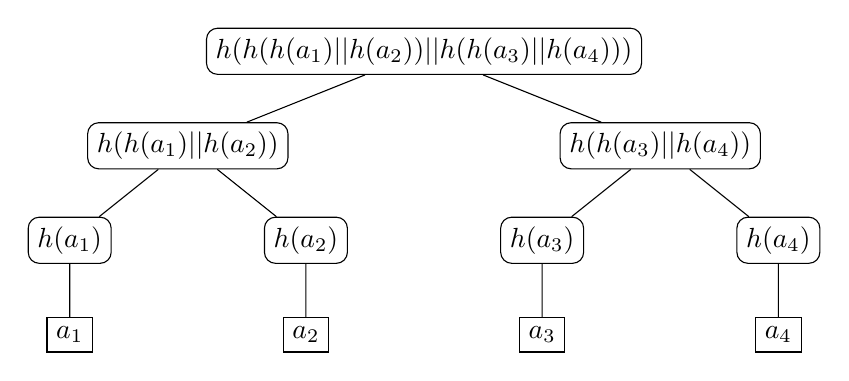
\begin{tikzpicture}[grow=south, sibling distance=20mm, level 1/.style={sibling distance=6cm},
  level 2/.style={sibling distance=3cm},level 3/.style={sibling distance=1.5cm}, level distance=12mm, every node/.style={draw=black, fill=none, rounded corners}]
  \node  {$h(h(h(a_1)||h(a_2))||h(h(a_3)||h(a_4)) )$} 
        child { node {$h(h(a_1)||h(a_2))$}
            child {node {$h(a_1)$}
                child {node[rounded corners=0pt] {$a_1$}}
            }
            child {node {$h(a_2)$}
                child {node[rounded corners=0pt] {$a_2$}}
            }
        }
        child { node {$h(h(a_3)||h(a_4))$}
            child {node {$h(a_3)$}
                child {node[rounded corners=0pt] {$a_3$}}
            }
            child {node {$h(a_4)$}
                child {node[rounded corners=0pt] {$a_4$}}
            }
        };
\end{tikzpicture}
\caption{Merkle Tree de 3 niveles}
\label{fig:merkle_tree}

\end{figure}

Hay otras operaciones que nos interesan realizar sobre un Merkle Tree además de construirlo para obtener su raíz. Una de usos más comunes es \textbf{comprometerse a una lista} para luego revelar elementos a pedido sin revelar la lista entera. ¿Qué quiere decir esto?

Supongamos que un prover tiene una lista secreta $A$ de tamaño $N=2^n$ y necesita convencer a un verifier de que esa lista posee ciertos elementos en determinadas posiciones. Desde el punto de vista del verifier, quiere convencerse de que el prover tiene una lista $A$ con los elementos $e_1, \cdots, e_k$ en las posiciones $i=1,\cdots k$ ($k \leq N$). Para cada uno de estos elementos, el prover puede brindar una prueba criptográfica $\pi_{i,e_i}$. Veamos cómo es el protocolo:

\begin{enumerate}
    \item $Commit(A) \rightarrow [A]$: el prover computa el Merkle Tree de $A$ y le pasa al verifier la raíz del árbol, que va a funcionar como el commit o “huella digital'' de la lista $A$. Si asumimos que la función de hash se comporta como un oráculo aleatorio, entonces la probabilidad de que otra lista tenga la misma huella es casi nula. 
    \item $Open(A, i) \rightarrow a_i, \pi_{i,a_i}$: la idea acá es mandar un \textbf{camino de autenticación} de la posición $i$-esima. Para esto alcanza con mandar un nodo interno del árbol por nivel. ¿Cómo funciona esto? Consideremos una lista $A$ de largo $N=4$ como la de la figura \ref{fig:merkle_tree}. Supongamos que el verifier quiere conocer el valor de la posición $3$, es decir, $a_3$. ¿Cuáles son los valores que el prover tiene que darle para que pueda llegar hasta la raíz? En este caso, esos valores serían $\pi_{3,a_3} = h(a_4)$ y $h(h(a_1)||h(a_2))$. ¿Por qué es suficiente con esto? Veamos los pasos que realiza el verifier en la verificación.
    \item $Verify([A], i, a_i, \pi_{i, a_i}) \rightarrow \{true, false\}$: 
    \begin{enumerate}
        \item Calcula $h(a_3)$ a partir del valor obtenido de $a_3$. Recordemos que la función de hash es pública para el protocolo. 
        \item Teniendo $h(a_4)$ que fue provisto por el prover, puede calcular $h(h(a_3)||h(a_4))$.
        \item Teniendo $h(h(a_1)||h(a_2))$ que fue provisto por el prover, puede calcular \\ $h(h(h(a_1),h(a_2))||h(h(a_3),h(a_4)))$, habiendo llegado de esta manera hasta la raíz. Llamemos al valor obtenido de la raíz $[A]'$.
        \item Finalmente, verifica que $[A] = [A]'$ para convencerse de que efectivamente $a_3$ es el elemento en el índice $3$ de $A$.
    \end{enumerate}
    Notemos que la cantidad de pasos a realizar de forma recursiva es del orden de $n$, es decir, logarítmica respecto al tamaño de la lista o lineal respecto a la altura del árbol. Una representación del proceso de verificación puede verse en la figura \ref{fig:merkle_path}. En rojo están los valores provistos por el prover y en verde los valores calculados por el verifier (la raíz de el árbol entra en ambas categorías).
\end{enumerate}

\begin{figure}
\centering
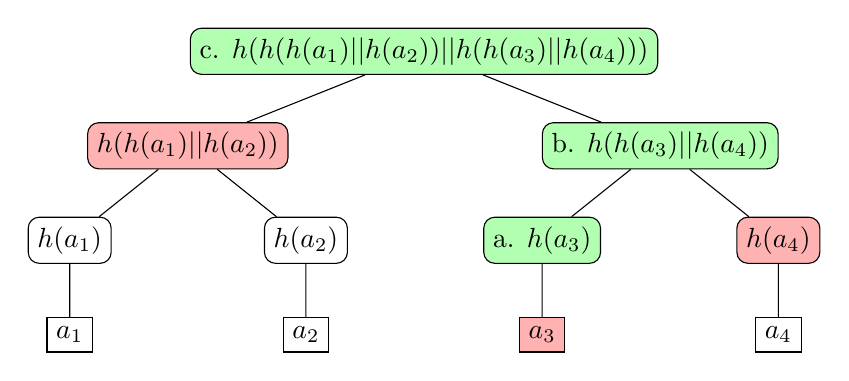
\begin{tikzpicture}[grow=south, sibling distance=20mm, level 1/.style={sibling distance=6cm},
  level 2/.style={sibling distance=3cm},level 3/.style={sibling distance=1.5cm}, level distance=12mm, every node/.style={draw=black, fill=none, rounded corners}]
  \node[fill=green!30]  {c. $h(h(h(a_1)||h(a_2))||h(h(a_3)||h(a_4)) )$} 
        child { node[fill=red!30] {$h(h(a_1)||h(a_2))$}
            child {node {$h(a_1)$}
                child {node[rounded corners=0pt] {$a_1$}}
            }
            child {node {$h(a_2)$}
                child {node[rounded corners=0pt] {$a_2$}}
            }
        }
        child { node[fill=green!30] {b. $h(h(a_3)||h(a_4))$}
            child {node[fill=green!30] {a. $h(a_3)$}
                child {node[fill=red!30, rounded corners=0pt] {$a_3$}}
            }
            child {node[fill=red!30] {$h(a_4)$}
                child {node[rounded corners=0pt] {$a_4$}}
            }
        };
\end{tikzpicture}
\caption{Merkle Path para $a_3$}
\label{fig:merkle_path}
\end{figure}

\section{FRI}
Otro protocolo que implementa oráculos de polinomios es FRI. Este protocolo tiene la ventaja de que no necesita un CRS para funcionar, sin embargo las pruebas que genera ocupan más espacio de almacenamiento que las de KZG para alcanzar el mismo nivel de seguridad. FRI también es un protocolo interactivo, con muchas más interacciones que KZG y que se apoya en los commitments de listas de los Merkle Trees vistos en la sección \ref{sec:merkle_tree}. 

Concretamente, FRI es una Low Degree Proof: un protocolo que sirve para demostrar que el prover conoce un polinomio de grado \textbf{menor estricto a} un cierto $N = 2^n$. El polinomial commitment scheme se apoya en este protocolo para dar garantías de Soundness. 

\subsection{Polinomial Commitment Scheme sobre FRI}
Nuevamente partimos de que el prover conoce un polinomio $p$ de grado $N = 2^n$ y quiere comprometerse a ese polinomio para que el verifier pueda abrirlo en algún punto que desee, convenciéndose de que la evaluación obtenida se corresponde al polinomio comprometido inicialmente. Vamos a comenzar tomando un valor $M = 2^{n+b}$, donde $b$ es un parámetro de seguridad (o \textit{blowup-factor}) y tomar una raíz M-ésima de la unidad $\omega$ para armar un dominio de evaluación

$$D=\{1, \omega, \omega ^2, \cdots, \omega ^{M-1}\}$$

El protocolo es como sigue:

\begin{enumerate}
    \item $Commit(p) \rightarrow [p]$: Lo primero que va a hacer el prover es inicializar un Merkle Tree con hojas $$[p(1), p(\omega),p(\omega^2),\cdots, p(\omega^{M-1})]$$
    De esta manera va a obtener un Merkle Hash de su raíz $[p]$, es decir, un Merkle Hash de las evaluaciones de $p$ en el dominio $D$. A continuación va a darle $[p]$ al verifier. 

    Podemos volver nuevamente a la abstracción de que el prover le está dando al verifier un oráculo de $p$, acotado a los valores del dominio $D$. 

    \item $Open(p, z) \rightarrow p(z)$: El verifier va a pedir la evaluación de $p$ en un valor $z \in D$, por lo tanto va a darle al prover ese valor. El prover va a retornar $p(z)$ al verifier. 
    
    \item $Verify([p], p(z))\rightarrow \{true, false\}$: El verifier va a pensar en el polinomio 
    
    $$q(x) = \frac{p(x) - p(z)}{x-z}$$
    
    No tiene acceso a este polinomio, sin embargo puede usar algo llamado \textit{oráculo virtual} (o $[q]$), obteniéndolo a través de $[p]$. Es decir, si el verifier puede obtener evaluaciones de $p$ usando el oráculo, también puede obtener evaluaciones de $q$ usando el mismo oráculo $[p]$. El truco para hacer la verificación es el siguiente: si efectivamente la evaluación que el prover dio de $p(z)$ es correcta, entonces $q$ debería tener un grado menos que $p$. Si la evaluación no es correcta, entonces $q$ va a tener un grado notablemente más alto. Al verifier le alcanza entonces con convencerse de que $q$ tiene grado \textit{a lo sumo} $N-1$ para ver que $p$ tiene grado $N$. Para garantizarse esto, va a recurrir al protocolo FRI explicado en el apéndice \ref{sec:fri_ldp}.
    
\end{enumerate}

Un detalle importante es que al aplicar la heurística de Fiat-Shamir, todo el protocolo FRI estará comprimido en una única prueba, armada de forma offchain por el prover. La verificación ocurre en tiempo succint. 

